\documentclass[nobib]{tufte-handout}

%\\geometry{showframe}% for debugging purposes -- displays the margins

\newcommand{\bra}[1]{\left(#1\right)}
\usepackage{amssymb}
\usepackage{hyperref}
\usepackage[activate={true,nocompatibility},final,tracking=true,kerning=true,spacing=true,factor=1100,stretch=10,shrink=10]{microtype}
\usepackage{color}
\usepackage{steinmetz}
% Fixes captions and images being cut off
\usepackage{marginfix}
\usepackage{array}
\usepackage{tikz}
\usepackage{amsmath,amsthm}
\usetikzlibrary{shapes}
\usetikzlibrary{positioning}
\usepackage{listings}
\usepackage{caption}
\usepackage{circuitikz}
\DeclareCaptionFont{white}{\color{white}}
\DeclareCaptionFormat{listing}{\colorbox{gray}{\parbox{\textwidth}{#1#2#3}}}
\captionsetup[lstlisting]{format=listing,labelfont=white,textfont=white}

% Set up the images/graphics package
\usepackage{graphicx}
\setkeys{Gin}{width=\linewidth,totalheight=\textheight,keepaspectratio}
\graphicspath{{.}}

\title{Notes for ECE 36200 - Microprocessor Systems and Interfacing}
\author[Shubham Saluja Kumar Agarwal]{Shubham Saluja Kumar Agarwal}
\date{\today}  % if the \date{} command is left out, the current date will be used

\usepackage{pgfplots}
% The following package makes prettier tables.  We're all about the bling!
\usepackage{booktabs}

% The units package provides nice, non-stacked fractions and better spacing
% for units.
\usepackage{units}

% The fancyvrb package lets us customize the formatting of verbatim
% environments.  We use a slightly smaller font.
\usepackage{fancyvrb}
\fvset{fontsize=\normalsize}

% Small sections of multiple columns
\usepackage{multicol}

% For finite state machines 
\usetikzlibrary{automata} % Import library for drawing automata
\usetikzlibrary{positioning} % ...positioning nodes
\usetikzlibrary{arrows} % ...customizing arrows
\tikzset{node distance=2.5cm, % Minimum distance between two nodes. Change if necessary.
    every state/.style={ % Sets the properties for each state
    semithick,
    fill=gray!10},
    initial text={}, % No label on start arrow
    double distance=2pt, % Adjust appearance of accept states
    every edge/.style={ % Sets the properties for each transition
    draw,
    ->,>=stealth', % Makes edges directed with bold arrowheads
    auto,
    semithick}}
\let\epsilon\varepsilon

% These commands are used to pretty-print LaTeX commands
\newcommand{\doccmd}[1]{\texttt{\textbackslash#1}}% command name -- adds backslash automatically
\newcommand{\docopt}[1]{\ensuremath{\langle}\textrm{\textit{#1}}\ensuremath{\rangle}}% optional command argument
\newcommand{\docarg}[1]{\textrm{\textit{#1}}}% (required) command argument
\newenvironment{docspec}{\begin{quote}\noindent}{\end{quote}}% command specification environment
\newcommand{\docenv}[1]{\textsf{#1}}% environment name
\newcommand{\docpkg}[1]{\texttt{#1}}% package name
\newcommand{\doccls}[1]{\texttt{#1}}% document class name
\newcommand{\docclsopt}[1]{\texttt{#1}}% document class option name

% Define a custom command for definitions and biconditional
\newcommand{\defn}[2]{\noindent\textbf{#1}:\ #2}
\let\biconditional\leftrightarrow

\begin{document}

\maketitle

\begin{abstract}
    These are lecture notes for spring 2024 ECE 36200 at Purdue as taught by Professor Younghyun Kim. Modify, use, and distribute as you please.
\end{abstract}

\tableofcontents

\newpage

\section{General-Purpose IO (GPIO)}
GPIO allows us to interface a microcontroller with the rest of the world.\\
These microcontrollers have a number of pins which can be written to and read from using software.\\
Some functions of microcontroller pins are:
\begin{itemize}
    \item Read to check if external voltages are applied.
    \item Apply a voltage to a pin.
    \item It can also perform Digital-to-Analog and Analog-to-Digital conversions.
    \item Several other functions are also available.
\end{itemize}
A GPIO has the following corresponding circuitry:
\begin{center}
    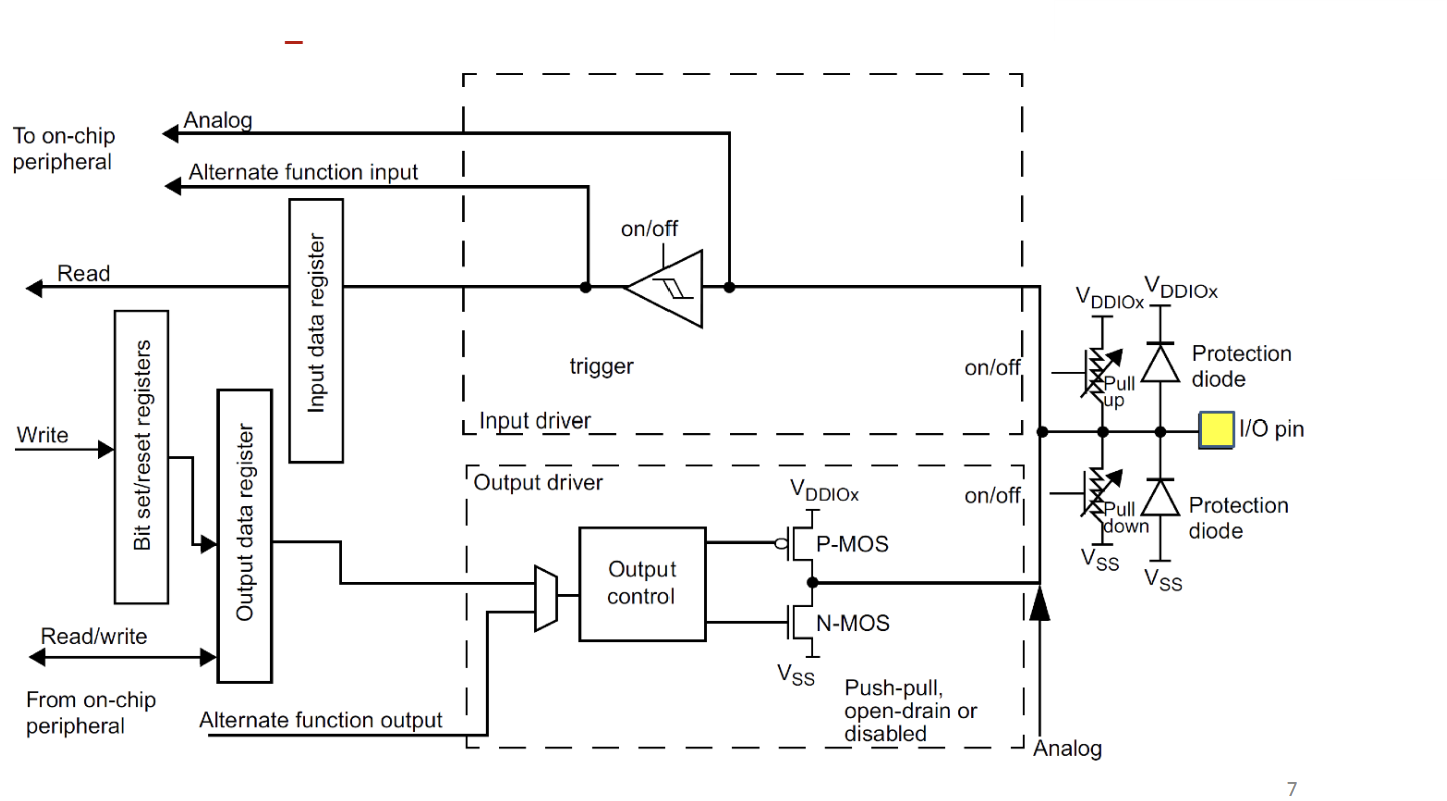
\includegraphics[width = 200px]{images/gpio_circuitry.png}
\end{center}
\subsection{Output}
The output is controlled by the following (push/pull configuration):
\begin{center}
    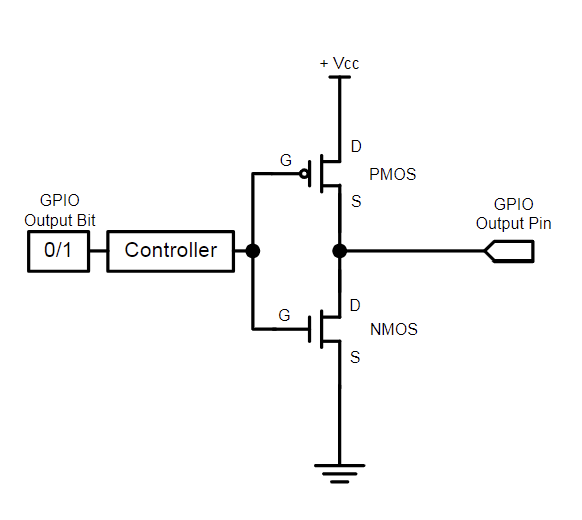
\includegraphics[width = 130px]{images/output control.png}
\end{center}
When the GPIO bit is 0, the output pin will have a 1, and vice versa. That is, it connects to the output with a NOT gate.\\
However, there are other methods as well, such as the following open drain circuit:
\begin{center}
    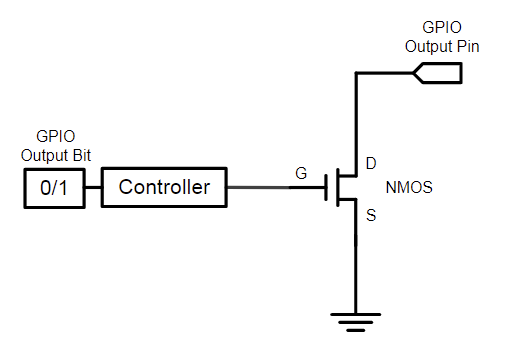
\includegraphics[width = 130px]{images/open_drain_output_control.png}
\end{center}
In this configuration, when the GPIO out is 0, the output will be 0 as well. However, if it is 1, the output will float. This thus requires a pull-up resistor to function.\\
\subsection{Control Speed}
On a slight side note, we will analyze speed control.
The tradeoffs of speed control are the following:
\begin{itemize}
    \item More GPIO speed $\implies$ more noise and more power consumption
\end{itemize}
Thus, the speed must be configured based on peripheral speed.\\
We can then relate the speed with the slew rate of the signal:\\ $slewrate = \max\left(\frac{\Delta V}{\Delta t}\right)$\\
\subsection{Input}
The following is the input control/read circuit: 
\begin{center}
    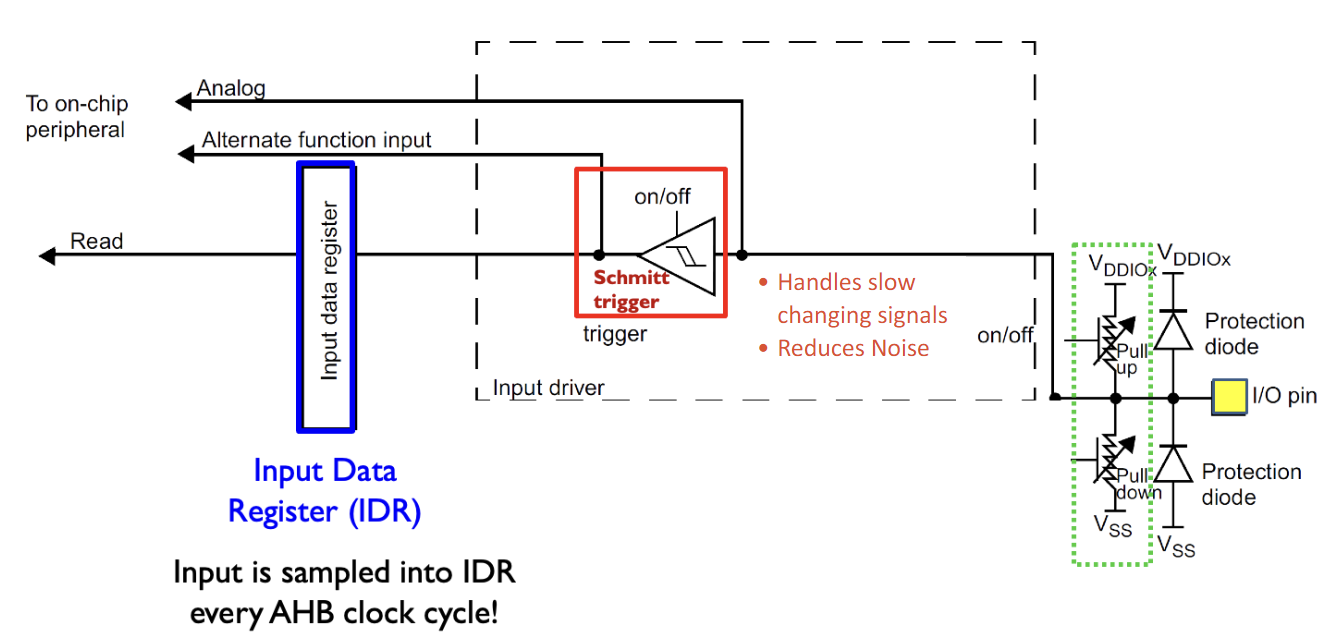
\includegraphics[width = 200px]{images/input_control.png}
\end{center}
The Schmitt trigger in the above circuit allows for noise control on the input.
A Schmitt trigger has two thresholds, restricting changes from 0 to 1 and from 1 to 0:
\begin{center}
    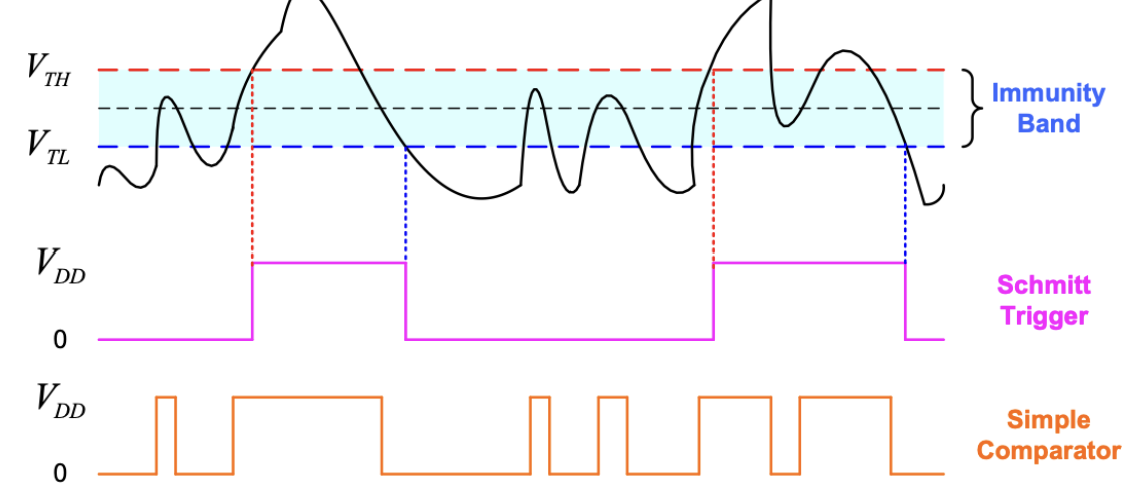
\includegraphics[width = 200px]{images/schmitt_example.png}
\end{center}
However, it should be noted that there exist quite a few electrical non-idealities, complicating input read procedures.\\
One solution for some of these problems is the use of the famous pull-up/pull-down  resistors.\\
The resistance values must be calculated. If it were too low, it would act as a short circuit, increasing power consumption. If it were too high, however, it would be very slow.\\
\subsection{Control}
There are two main options for IO control.:
\begin{enumerate}
    \item Special instructions in the processor.\\
    This is known as port-mapped IO, where each device is assigned a unique port number.
    \item Memory-mapped IO\\
    Each one is assigned a unique memory address.\\
    \textbf{IMPORTANT: For example, a 32-bit memory space has 1B long addresses.}\\
    This means the microcontrollers that are used in class, which are 32-bit have limited read/write memory ($2^{32}$B$\approx 4$GB).\\
    The memory can be allocated as follows:\\
    \begin{center}
        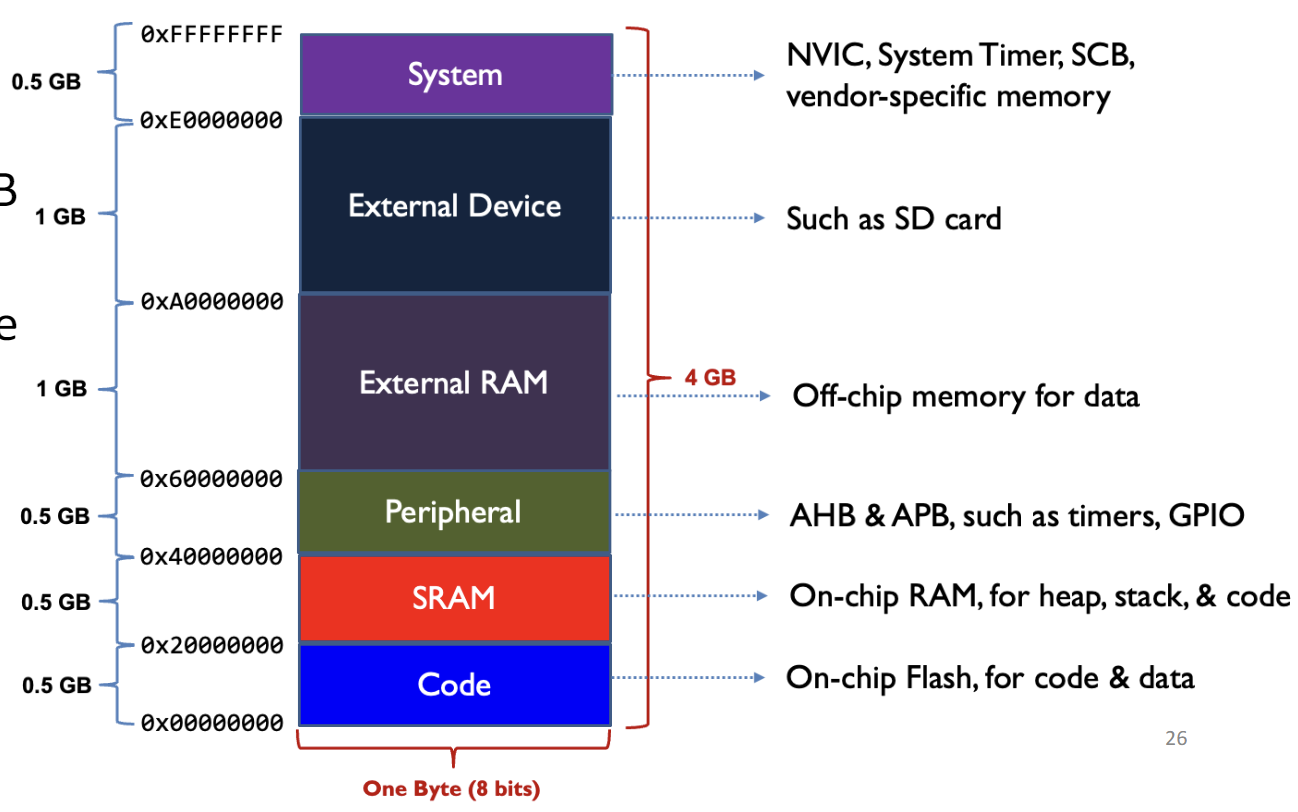
\includegraphics[width=200px]{images/memory_allocation.png}
    \end{center}
\end{enumerate}
\subsection{Memory Types}
\begin{itemize}
    \item SRAM (Static Random Access Memory)
    \begin{itemize}
        \item Volatile
        \item Variables
        \item Stack 
        \item Buffers
        \item Test Code
    \end{itemize}
    \item Flash Memory 
    \begin{itemize}
        \item Non-Volatile
        \item App Code
        \item Static Data 
        \item Vectors (resets and interrupts)
    \end{itemize}
\end{itemize}
\subsection{Microprocessor Interfacing}
A CPU reads from RAM to read/write variables.\\
It reads from ROM which contains read-only data.\\
It uses a bus to drive the address.\\
Another bus is used to send or receive data.\\
All GPIO peripherals have their own addresses, and can thus be accessed similar to the memory.\\
GPIO control needs to control both the Direction Register and the Data Register.\\
\textit{Note: memory is accessed at a minimum granularity of 1B, but more commonly 4B.}\\
\subsection{Conclusion}
GPIO can do pretty much anything, given enough pins.\\
It uses bus protocols to implement these processes.\\
\section{Interrupts}
An interrupt is generated by hardware or software to inform that a condition has been fulfilled.\\
Interrupts have an advantage over forever loops in that the conditions are not checked in every loop, making the whole program far more efficient.\\
An interrupt is a type of exception.\\
\defn{Exception}{hardware invoked subroutine}\\
\subsection{Program Counter}
The code defined by your program is stored in memory as a series of binary values.\\
To keep track of location in code, called Program Counter, or PC.\\
PC is an address that points to the next command to be run.\\
\subsection{Basics}
Peripherals can raise interrupts.\\
The CPU can be interrupted by more than one thing, that is, more than one kind of interrupt.\\
The interrupts are linked to functions (Interrupt Service Routines) stored in a vector table.\\
These interrupts can be enabled and disabled, permitting or preventing peripheral from raising interrupts.\\
Interrupts have priorites, that is, a higher priority interrupt can interrupt a lower priority interrupt, but not the other way around.\\
When interrupts are raised, they are not immediately handled, but are instead placed into a sort of pending queue.\\
The following is the flow of an interrupt:\\
\begin{enumerate}
    \item Peripheral raises an interrupt
    \item CPU checks if this is enabled
    \item CPU marks it as pending
    \item Checks priority against current priority level (CPL), and runs if highest
    \item If the priority is the highest:
    \begin{itemize}
        \item Update CPL to this priority
        \item Push CPU to stack
        \item Push this entry into vector table on PC
    \end{itemize}
    \item The ISR should now be running
\end{enumerate}
Tables like the ISR vector table are stored in the hardware, and modified or accessed using memory locations through direct access.\\
Only vector table lookup and stack saving require the memory to be accessed.\\
When interrupted, the CPU stores the current state (to return to later) into the SRAM. This information is retrieved once the interrupt is fulfilled.\\
Interrupts are usually handled at the end of a line of instruction. The code later continues at the line right after it.\\
If a fault happen sin the middle of an interrupt, the resume is at the same interrupt.\\
Interrupts are expected to be quick.\\
Interrupts also require specialized hardware to effectively interrupt the CPU.\\
\section{Basic Timers, Debouncing, Multiplexing}
Timers are a piece of hardware that allow us to execute tasks periodically.\\
Any useful microcontroller has a rich hardware system.\\
A System Ticker is a "special" timer used for system specific tasks.\\
A timer causes the CPU to execute a task, after every interval T.\\~\\


SysTick Interrupt Time Period = (SysTick Load Period + 1) $\times$ 
\end{document}

